\chapter{Torque Limit Considerations}
\label{ch:envparams}

Much effort in reinforcement learning has been spent on finding better or faster algorithms that can solve any \ac{RL} problem in a model-free way, i.e. only through interactions with the environment. However, most success stories, such as TD-Gammon~\cite{tdgammon} and AlphaGo~\cite{alphago}, still required careful engineering. Therefore, we believe that the design of the character and the tasks can be in some cases far more important to achieving superior results than the algorithm itself. In other words, making the problem itself simpler and more compatible with the algorithm used can be more productive than finding new algorithms that claim to solve more difficult problems. In this chapter, we look at the effects of different \ac{TL} settings and we show that a simple torque limit curriculum can help achieve higher rewards and more reliable results.

\section{Introduction}
\label{sec:params_torque}

To measure the strength of a person we can measure the strength of his/her muscles. Similarly, we can measure the strength of a robot by measuring the strength of its motors. To do this, we need to consider each joint separately. A natural measure of strength is the amount of torque that the joint can produce. Furthermore, as ideal robots are consistent and never get tired like humans do, we only need to measure the maximum amount of torque output. Hence, a standard way of representing robot strength is through a \ac{TL} vector. Naturally, a simulated character modelled after a robot needs to have a pre-specified \ac{TL}. The correctness of \ac{TL} is of high importance as it determines the capabilities of the robot. Having a higher or lower \ac{TL} setting, therefore, has serious implications on what the agent can or cannot do and how quickly or more reliably the task can be solved.

Experimenting in a simulator, however, allows us to use torque limits that are much higher or lower than in real life and to investigate their effects. In most applications, lower limits tend to be more desirable. In robotics, using excessive forces can cause damage to the robot as well as its surroundings including any human or animals that may be in its vicinity. Using a low torque limit can be seen as a simple but effective safety mechanism that can alleviate many problems. The consequences of using unrealistic limits in computer graphics may not be as dire, but humans are good at perceiving inconsistent movements performed by human-like characters. An impossibly high jump, pushing a heavy object with one hand, and recovering from a fall by using excessive strength are all immediately recognizable by a human observer. Low limits, on the other hand, are usually not noticeable unless the character or robot fails to accomplish the task at hand, as people rarely ever use maximum strength for day to day tasks.

Consequently, researchers in robotics and computer graphics tend to care about using realistic limits on the characters. On the other hand, the machine learning community is usually less concerned with such details and tends to use characters with excessive \ac{TL}. This has been a source of (informal) complaints from the aforementioned communities.

One common way of compelling the agent to use less force is via an energy consumption cost. This approach is widely used in practice. However, it has two disadvantages. First, the agent can still use excessive force if it so desires. More importantly, the energy consumption can be harmful for training. Therefore, the weight of the energy consumption cost is set low enough that it may be ignored by the agent \cite{Yu-SIGGRAPH-2018}.

We aim to solve both of these problems by using \ac{TL} as hard constraints. As a result, this chapter aims to answer the following questions: how much does the torque limit affect learning and can we make use of this knowledge to find better solutions?

Our results indicate that \ac{TL} settings strongly affect the final solution. Below a certain threshold, the learning algorithm generally fails to find any solution, in a reasonable amount of time, that can solve the task. We demonstrate that this phenomenon is not a consequence of the problem setup but rather a limitation of the optimization procedure by showing the existence of higher-performing solutions with the same setting. Finally, we offer a simple solution to fix this problem by using a curriculum during learning. This helps the agent to learn in a simpler environment and then transfer the learned solution to the more difficult setting.

\section{Environments}

We experiment with a set of existing locomotion environments from  Roboschool~\cite{ref:roboschool}. All characters are simulated using PyBullet~\cite{ref:Pybullet} which is a Python interface for the Bullet3 physics engine. In all of the environments, the task is for the character to walk as far as possible in the forward direction in the allotted time. The reward function also includes terms to encourage the agent to use less energy and stay ``alive'' longer, i.e. to not fall. The observation space in all of these environments consists of root information (root z-coordinate, x and y heading vector, root velocity, roll, and pitch), joint angles, joint angular velocities, and binary foot contact information. The torques are all normalized between $-1$ and $1$.

\bfpara{Walker2D} is a simplified bipedal character whose movements are constrained to a 2D plane. An action is a 6D vector corresponding to torques at the hip, knee, and ankle on both left and right legs. The observation space is 22D and it weighs about 24kg.

\bfpara{Hopper} is a one-legged character constrained to a 2D plane. It is similar to the Walker2D with one leg missing. The action space is 3D where each dimension controls the torque at the hip, knee, and ankle. The observation space is 15D and it weights about 16jg.

\bfpara{HalfCheetah} is a 2D model that closely resembles a quadruped with only a fore and a hind left (no sides). An action is a 6D vector, similar to Walker2D, corresponding to the normalized torques at the thigh, shin, and the foot for each of the fore and hind legs. The observation space is 26D and consists of the same information as Walker2D with the addition of more fine-grained contact information. The character weighs about 38kg.

\bfpara{Ant} is a 3D character that resembles an insect with four legs. It consists of a torso as well as four legs that are each divided into two segments. The action space is 8D and the observation space is 28D containing the same information as Walker2D. Despite being three dimensional, this character is highly stable due to having four legs. The character weighs about 182kg.


\section{Methods}

To experiment with different torque limits we need a way to dynamically modify the limits in each environment. Therefore we slightly modified the aforementioned environments to include a parameter denoted by the \ac{TLM}. \ac{TLM} is a single scalar variable and the torque limits are altogether multiplied by this shared scalar which lets us shrink or expand the limits all at once. It is possible to have a specific multiplier for each joint, however, a single variable is sufficient for the purposes of our work.

We use our implementation of PPO \cite{ppo} for all the experiments\footnote{The source code is available at \url{https://github.com/farzadab/walking-benchmark}}.
The hyper-parameters used can be found in \Cref{sec:envparam_hyperparams}.
Each experiment collected 6 million environment time steps in total and all the experiments were replicated five times each.


% \red{Comment on whether the current limits are realistic or how far they are from reality  +++  mention that Roboschool already has more realistic than MuJoCo.}

% \red{\url{https://www.researchgate.net/figure/Joint-torque-and-power-for-human-hip-knee-and-ankle-in-treadmill-walking-Joint-torques_fig1_272484378}}

% \red{thigh and knee both have a default of 100 Nm, whereas ankle is at 30 Nm}

\section{Results}

In this section, we begin by demonstrating the effect of torque limit on training and then provide a more appropriate way of enforcing this limit.
All plots in this section report the average performance as well as the minimum and maximum across five runs.

\subsection{Torque Limit Baseline Experiments}

To determine how the torque limit can affect the final solution, we run a set of experiments on the Walker2D environment with different values of $TLM$ specified. To rule out the effect of random noise which is an important contributing factor in \ac{DRL} experiments \cite{rl_that_matters} we run each experiment five times with different random seeds and the mean of the data is reported as well as the best and the worst results.

\begin{figure}
    \centering
    \begin{subfigure}[t]{\textwidth}
        \centering
        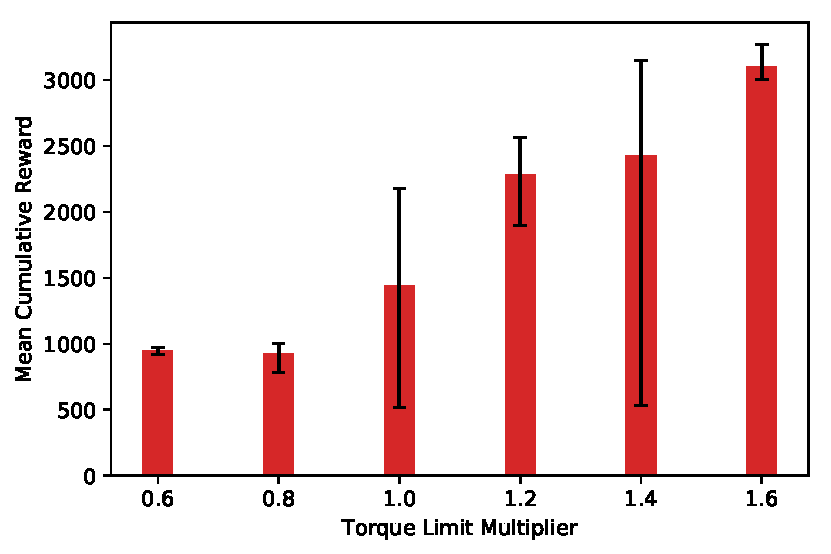
\includegraphics[width=90mm]{img/TorqueLimit_Reward.pdf}
        \caption{Cumulative rewards}
    \end{subfigure}
    \begin{subfigure}[t]{\textwidth}
        \centering
        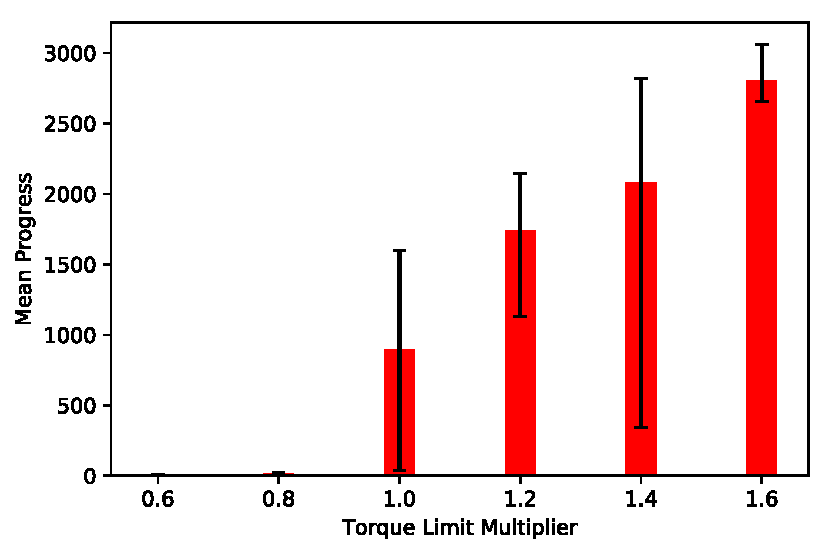
\includegraphics[width=90mm]{img/TorqueLimit_Progress.pdf}
        \caption{Amount of progress in each iteration}
        \label{fig:torque_limit_base_b}
    \end{subfigure}
    \caption{Final performance of the agent with different \ac{TLM} values.}{The error bars reflect the best and the worst performance achieved by the same algorithm over five runs with different random seeds.}
    \label{fig:torque_limit_base}
\end{figure}

The final cumulative return, as well as the amount of progress made at test time, are shown in \Cref{fig:torque_limit_base}. Not surprisingly the agents that had a higher torque limit constraint achieved higher returns. Interestingly, below a certain point (all runs with $TLM \leq 0.8$ as well as some runs with $TLM=1$) the agent failed to make any forward progress. Note that the cumulative return in these cases is still as high as one thousand. This is the result of the agent learning to stand still and avoiding early termination instead of learning to walk.

The results for the default torque limit ($TLM=1$ in the same figure) show us something interesting. First, the variance in the results is high. This is a known problem of reinforcement learning algorithms \cite{rl_that_matters}. More importantly, this hints at the existence of a local optimum where the agent does not learn to move and just avoids early termination by standing still. Even though the results of training with higher torque limits show variations as well, none of them seem to be stuck in this local optima. Lastly, the results seem to indicate that it is not possible to walk with the lower torque limits of 0.6 and 0.8.

\subsection{Torque Limit Curriculum}
If our hypothesis is correct that the agents are getting stuck in a local optimum with lower torque limits, it may be possible to get a better controller simply by using a better initialization. Agents trained with higher torque limits can intuitively provide a good starting point. This leads us to \textit{curriculum learning} \cite{Bengio:2009:CL:1553374.1553380}.

Curriculum learning is motivated by how humans and animals learn and is based on the idea of learning gradually from simple concepts to more difficult ones. In this approach, instead of training on the most difficult version of the problem, the training is divided into multiple stages where the first stage is a simplified version of the problem and task becomes more difficult at each stage until the last stage in which the agent is faced with the original version of the problem.

According to \Cref{fig:torque_limit_base}, tasks with higher torque limits seem to be easier to solve. Therefore, we can define a curriculum where the agent first sees high torque limit environments but gradually the limit is lowered linearly until it matches our final target. To make the training more stationary the training is divided into several levels during which \ac{TLM} stays fixed. The number of these levels is a hyper-parameter denoted by $NLevels$. For most experiments we used $NLevels=10$.

The results of applying the torque limit curriculum can be seen in \Cref{fig:torque_limit_curr}. This method not only achieves higher performance, it also manages to sidestep the local optima as evident in \Cref{fig:torque_limit_curr_b}. As a bonus, this approach seems to be more reliable in most cases as its variance seems to be lower than the baseline approach, except at $TLM=0.6$. In the latter case, the baseline always converges to the local optima which has relatively low variance, however, this is not the desired behaviour.


\begin{figure}
    \centering
    \begin{subfigure}[t]{\textwidth}
        \centering
        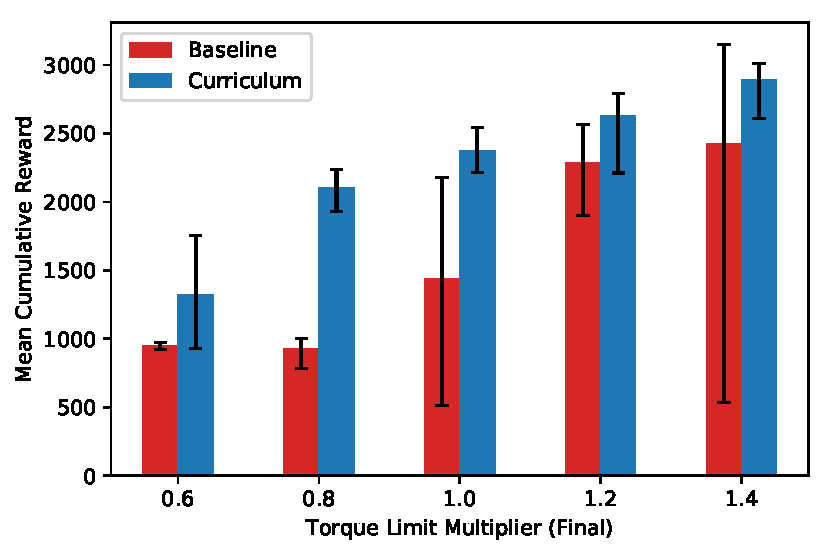
\includegraphics[width=90mm]{img/TorqueLimit_Curr_Reward.pdf}
        \caption{Cumulative rewards}
    \end{subfigure}
    \begin{subfigure}[t]{\textwidth}
        \centering
        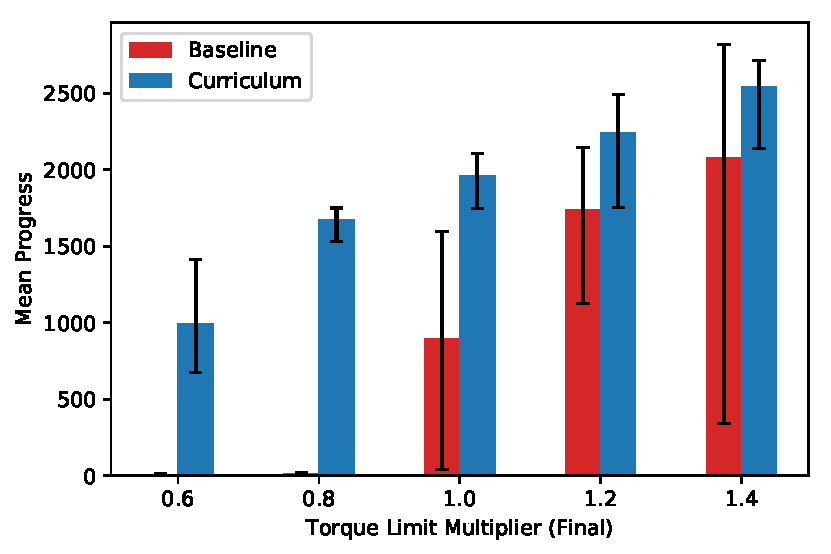
\includegraphics[width=90mm]{img/TorqueLimit_Curr_Progress.pdf}
        \caption{Amount of progress in each iteration}
        \label{fig:torque_limit_curr_b}
    \end{subfigure}
    \caption{The effect of curriculum learning for Walker2D.}{Blue plots show the final performance of the agents which started out with $TLM=1.6$ and the \ac{TLM} was decreased to the target value in ten steps. The red bars are the same as in \Cref{fig:torque_limit_base}.}
    \label{fig:torque_limit_curr}
\end{figure}


\subsection{Ablation and More Environments}

To further validate our approach, we test it on the Half Cheetah, Ant, and Hopper environments as well. As a baseline, we keep \ac{TLM} fixed at the target value.
Also, we compare our results with another curriculum approach that is very similar to our own, namely, an exploration rate curriculum, where the \ac{TLM} is kept fixed the same as in our baseline.
In this approach, the amount of exploration noise is varied at training time by starting at a high value to explore the solution space well and annealing it to a lower value in order to increase the final motion quality.

The results are shown in \Cref{fig:torque_limit_envs}. All experiments used the same hyper-parameters, namely with $NLevels=10$ and the \ac{TLM} going from $1.2$ to $0.6$. The exploration curriculum seems to be helpful to some extent but the \ac{TLM} curriculum works best for all environments, specifically for the Ant.

\begin{figure}
    \centering
    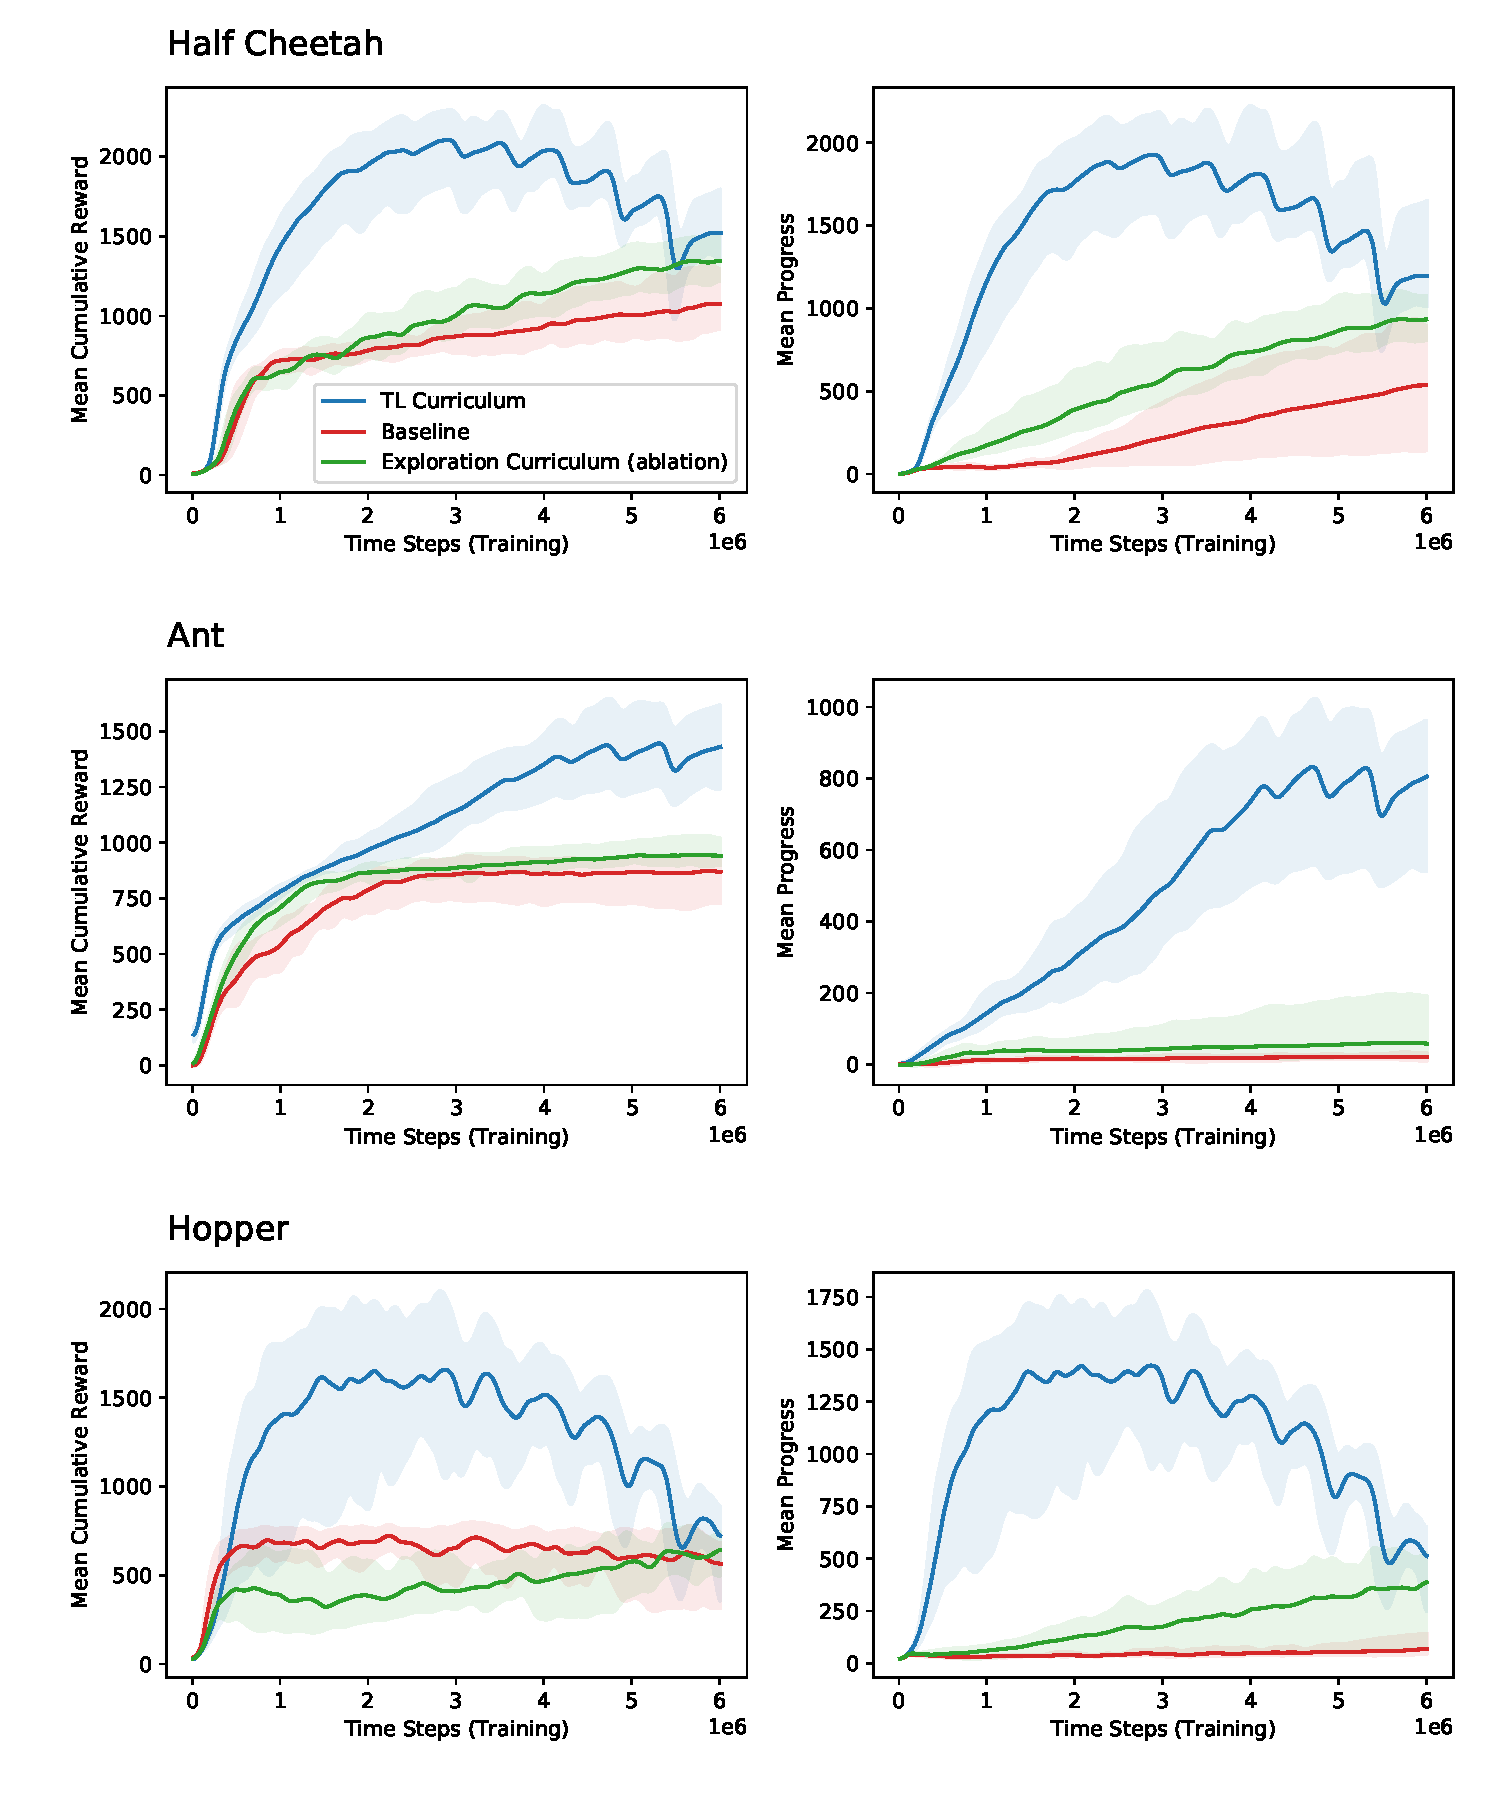
\includegraphics[width=130mm]{img/TorqueLimit_Envs.pdf}
    \caption{Torque limit curriculum results for Half Cheetah, Ant, and Hopper.}{The dips in performance reveal the points in which the value of \ac{TLM} was reduced. The final \ac{TLM} is constant across all methods. The shaded area corresponds to the minimum and the maximum values across five runs.}
    \label{fig:torque_limit_envs}
\end{figure}

\subsection{Curriculum Sensitivity}
\label{subsec:curr_sensitivity}

This curriculum learning technique seems to be useful in the different environments that we tested on, even though the gains vary across domains. However, as with many approaches, this method also includes hyper-parameters that need to be chosen by the user. We can assume that the target torque limits are a given, but the starting limits are not fixed. Furthermore, the optimal value for the \textit{NLevels} hyper-parameter is also unknown. An important question to ask is: how sensitive is this method to the hyper-parameters. Therefore, we designed two experiments to answer this question.

First, we look at the starting \ac{TLM}. We assume that the final \ac{TLM} of $0.6$ is fixed and we can vary the starting \ac{TLM} value. The results of the experiment on the Walker2D environment can be seen in \Cref{fig:torque_limit_hp_tlm}. Surprisingly, all initial values seem to work relatively well. Specifically, by comparing the results for $TLM=0.8$ with \Cref{fig:torque_limit_base_b}, we see that the final performance has increased instead of decreasing even though the final $TLM$ has decreased. This might simply be due to randomness, but it is also possible that the sudden changes in curriculum training let the agent escape local optima regions more easily. More importantly, the results seem to indicate that the method is not sensitive to this hyper-parameter as long as the initial \ac{TLM} value is high enough to stumble upon a good solution.

\begin{figure}
    \centering
    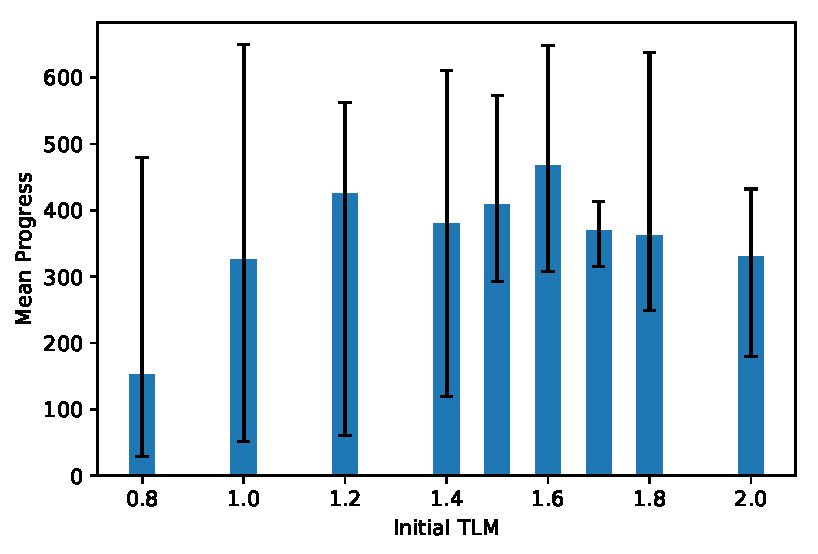
\includegraphics[width=90mm]{img/TorqueLimit_Curr_TLM.pdf}
    \caption{Curriculum sensitivity to initial \ac{TLM} value.}{All experiments with $TLM > 1.2$ have an acceptable performance both in terms of the average as well as the worse performance.}
    \label{fig:torque_limit_hp_tlm}
\end{figure}

Next, we look at the number of curriculum steps required, while keeping the total number of simulation steps fixed. A low number means an abrupt change but a high number would mean changing slowly but frequently. Both approaches have their merits. Changing slowly means the previous solution will still work under the new conditions, but it also means that there might not be enough time to get adjusted to the new situation before the next change. Abrupt changes can also be useful for getting out of a local solution. Again, we run a similar experiment as before on the Walker2D environment with the \ac{TLM} going from $1.6$ to $0.6$ with different number of steps. The results are provided in \Cref{fig:torque_limit_hp_steps}.

\begin{figure}
    \centering
    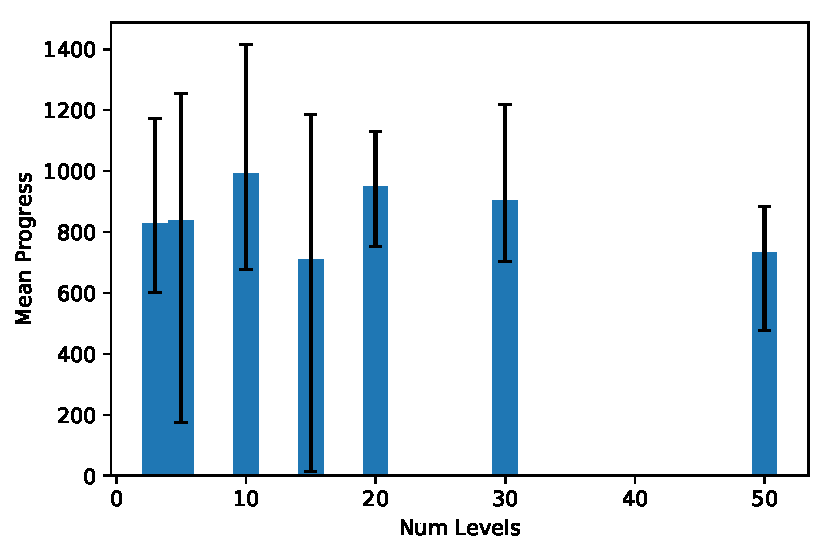
\includegraphics[width=90mm]{img/TorqueLimit_Curr_Steps.pdf}
    \caption{Curriculum sensitivity to the number of steps.}
    \label{fig:torque_limit_hp_steps}
\end{figure}

The results in both cases show some variability, which is to be expected, but there is no clear winner or a general trend to be pointed out. This is reassuring, as it shows that the method is not sensitive to small hyper-parameter changes. This makes the method more easily applicable to different settings.



\section{Conclusions}
In this chapter, we showed that the construction and the details of the locomotion environment are important, and the best design for learning need not be the most realistic one. Here, we looked at the effects of torque limits on learning. Torque limits describe how strong the character is and indirectly decides which movements are possible and which ones are not. The robotics and computer graphics communities tend to specify torque limits based on real-life robots and animals, but the machine learning community is less concerned with such details.

The torque limit setting is indeed important, as evident by the decrease in the final performance achieved in different settings. Furthermore, we show that this setting is specifically important in the context of reinforcement learning since with more restrictive configurations the learner tends to get stuck in local optima regions increasingly often. Therefore doing the initial training with higher torque limits is useful for sidestepping local optima and the resulting policy is perhaps more robust as a result of experiencing slightly different versions of the same environment.

